\beginsong{Am Ural}[
    wuw={axi (Alexej Stachowitsch)}, 
    bo={18}, 
    pfii={46}, 
    siru={15},
]

\beginverse
\endverse
\centering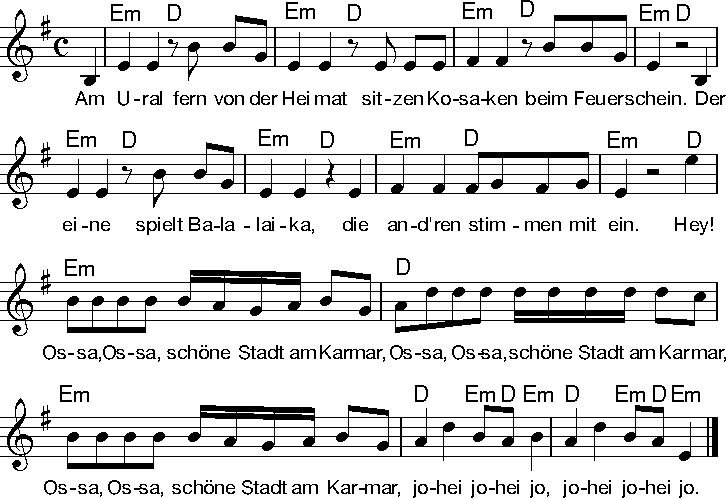
\includegraphics[width=1\textwidth]{Noten/Lied004.pdf}	

\beginverse
Am \[Em]Himmel, \[D]da leuchten die \[Em]Sterne, \[D] der \[Em]Wolf heult \[D]im finst'ren \[Em]Tal. \[D]
Die \[Em]Heimat, \[D]du grüßt sie von \[Em]Ferne, \[D] ver\[Em]gessen \[D]ist all' ihre \[Em]Qual! \[D]Hey!
\endverse

\beginchorus
\[Em]Ossa, Ossa, schöne Stadt am Karmar, \[D]Ossa, Ossa, schöne Stadt am Karmar,
\[Em]Ossa, Ossa, schöne Stadt am Karmar, \lrep \[D]Jo-hei, \[Em]jo-\[D]hei-\[Em]jo! \rrep
\endchorus
 
\beginverse
Die ^Pferde ^hell spitzen die ^Ohren, ^wenn die Ko^saken ^jauchzen und ^schrein. ^
Sie ^geben ^den Pferden die ^Sporen ^drüben am ^Wasser ^im Feuer^schein. ^Hey!
\endverse

\endsong
%\beginscripture{}
%Kosaken = Gemeinschaften freier Reiterverbände, zu denen sich flüchtige Russen und Ukrainer, manchmal auch nur Abenteurer %oder anderweitig Abtrünnige, in den südlichen Steppengebieten zusammenschlossen.
%\endscripture
